\documentclass[12pt]{report}
\usepackage[utf8]{inputenc}
\usepackage{graphicx}
\usepackage[english]{babel}
\usepackage[left=1.5in, right=1.5in, top=1in, bottom=1in]{geometry}
\graphicspath{ {D:/licenta/sounds/paper/images/} }
\usepackage{mathptmx}
\usepackage[nottoc,notlot,notlof]{tocbibind}


\begin{document}

\title{%
  Audio steganography \\
  \large High frequency message encoding \\
    exploiting human hearing}

\author{Teodor Paius, coord. Septimiu Crivei}

\maketitle

\begin{abstract}
Steganography is the practice of concealing a file, message, image, or video within another file, message, image, or video. This paper will focus on the domain of digital signal processing and audio concealment of messages. Apart from other common environments such as images or plain text, sound also represents a good way of transmiting hidden messages. The techniques present in this thesis can be applied not only to the target range of human hearing but can also be implemented with some degree of resemblance to other domains of higher frequencies (radio waves or elctro-magnetic waves).
\end{abstract}

\tableofcontents


\chapter{Introduction}
\section{Motivation}
Apart being a chance to delve deeper into a domain of computer science where i had previously less experience, this work was also developed with the ideea of improving existent security systems in mind. The sounds and how computers "recognize" them present on one had an interesting challenge to make effective use of them to hide messages, and on the other hand a good way of combining the robustness of mathematical methods with the huge processing power of today's computers.
\section{Context}
Today we live in a world where data confidentiality is of utmost importance. While the techniques of cryptography offer far more security potential than plain steganography, the existence of encrypted messages is obvious for an attacker, so attacks are inevitable. A good practice would be to hide this message, being them encrypted or not. This is where steganography could have an impact. As symetric key cryptography the strength of a technique lies in a secret know to both parties that take part in a communication. Of course some steganographic techniques have weaker hiding systems ( Least significant byte method ) than others ( phase coding or high frequency encoding ). By hiding the message it  wouldn't present and immediate chance for an attacker as file such images or audio are sent over the internet with millions each hour.
\section{Objective}
The objective of this work is to study in more detail an area of the art of steganography which is not as frequently used as it should be, and to create an effective way of hiding messages in sound in such a manner that only the sender and the receiver of the message could know to decode. This should consist in a method which has different variable parameters that can be send in advance between the participants of the conversation using similar techniques like the know key exchange methods used in everyday cryptography systems such as AES or DES/3DES. 
\section{Structure}
This project consists of a theoretical overview of the current steganographic techniques and the description of an algorithm which makes use of high frequency noise to hide certain messages, together with a practical application developed in Python to support the claims made in this report. 



\chapter{Theoretical background}

The commonly stated range of human hearing is 20 Hz to 20 kHz. Under ideal laboratory conditions, humans can hear sound as low as 12 Hz and as high as 28 kHz, though the threshold increases sharply at 15 kHz in adults, corresponding to the last auditory channel of the cochlea. Humans are most sensitive to (i.e. able to discern at lowest intensity) frequencies between 2,000 and 5,000 Hz. Based on this a good way of hiding information is exploiting this human weakness and encoding certain messages in audio files disguised as short sequences of high frequency signals.




\section{Overview of steganography}
The word steganography comes from the greek language being derived from the two greek words \emph{steganos}(covered) and \emph{graphein}(to write) referring to the art of enabling communication that uses methods of hiding information in plain sight. In the field of computer science steganography is the practice of concealing a file, message, image, or video within another file, message, image, or video.
The advantage of steganography over cryptography alone is that the intended secret message does not attract attention to itself as an object of scrutiny. Plainly visible encrypted messages, no matter how unbreakable they are, arouse interest and may in themselves be incriminating in countries in which encryption is illegal.\cite{note4}

The process of detecting certain messages hidden inside a stego-object (image, sound, video, etc.) is called steganalysis. The goal of steganalysis is to identify suspected packages, determine whether or not they have a payload encoded into them, and, if possible, recover that payload. 
Unlike cryptanalysis, in which intercepted data contains a message (though that message is encrypted), steganalysis generally starts with a pile of suspect data files, but little information about which of the files, if any, contain a payload. The steganalyst is usually something of a forensic statistician, and must start by reducing this set of data files (which is often quite large; in many cases, it may be the entire set of files on a computer) to the subset most likely to have been altered.

Usual methods of steganalysis consist in structural detection - difference in file properties(size, checksum, headers) or in statistical detection - changes in patterns of bits, LSB changes or hystogram analysis.

The algorithm proposed in this paper was designed in order to reduce the efficiency of such methods and to limit to possibility of detection caused by noticeable changes in file structure or composition, or by the appereance of anomalies in the stego-object.

\section{Overview of digital signal processing}
\subsection{Sound}
In physics, sound is a vibration transmitted through different enviroments: solid, gas or liguids. Sound can be divided mostly in two parts: pressure and time. These two are the characteristic of every wave and because of this a sound can be considered as a continous wave. Human ear, through its mechanisms, "catches" this stimulus and converts it in electrical signals which are sent to the brain to be analysed. This process is not perfect and this is the key fact on which this method relies.

Although there are many complexities regarding sound transmission, most of the time sound can be characterized by the following properties:
\begin{itemize}
	\item Frequency
	\item Amplitude
	\item Speed of sound
	\item Direction
\end{itemize}
In this method we are interested just in the first two properties: frequency and amplitude.

\subsection{DSP(Digital sound processing)}
To be able to analyze an analog(continous) signal in a digital environment, it must firstly be converted using and analog-to-digital converter. This process is composed of 2 major stages: discretization and quantization. This would transform a continous signal in a set of consecutive frames equidistant in time, and characterized by a certain amplitude. This also know as time domain. It is used to better visualize the overall image of a sound described as a wave. In (fig \ref{fig:samp_rate}) we can observe the discretization of a sinusoidal wave.

Another domain that is of significant importance to us is the frequency domain. Usually to change the time domain into frequency domain, a Fourier transform is applied over the discrete samples of the sound. This process converts the time domain samples into frequencies and amplitudes (fig \ref{fig:fourier}).

\begin{center}
\begin{math}
F\left(\zeta \right)\:=\:\int _{-\infty }^{\infty }\:f\left(x\right)e^{-2\pi x\zeta }
\end{math}
\end{center}


\begin{figure}
\centering
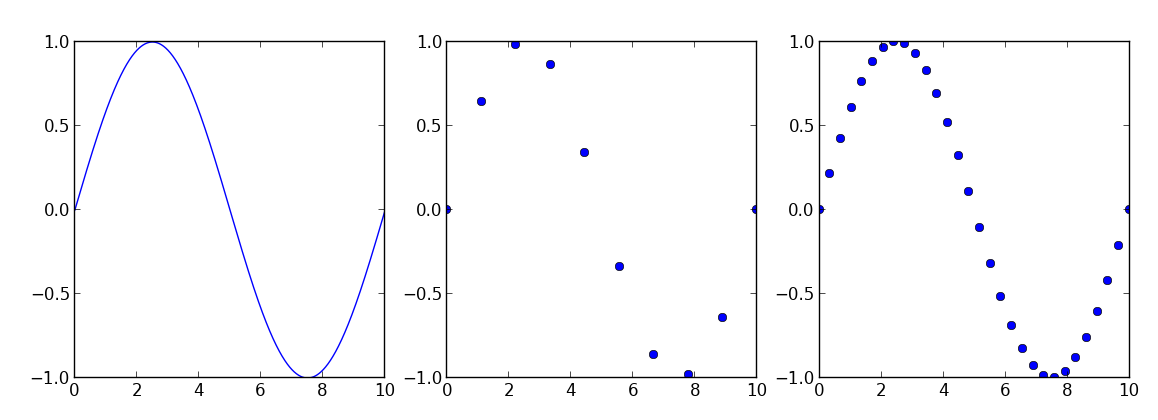
\includegraphics[width=1\textwidth]{sampling_rate}
\caption{Continous signal splitted in discrete samples}
\label{fig:samp_rate}
\end{figure}

\begin{figure}
\centering
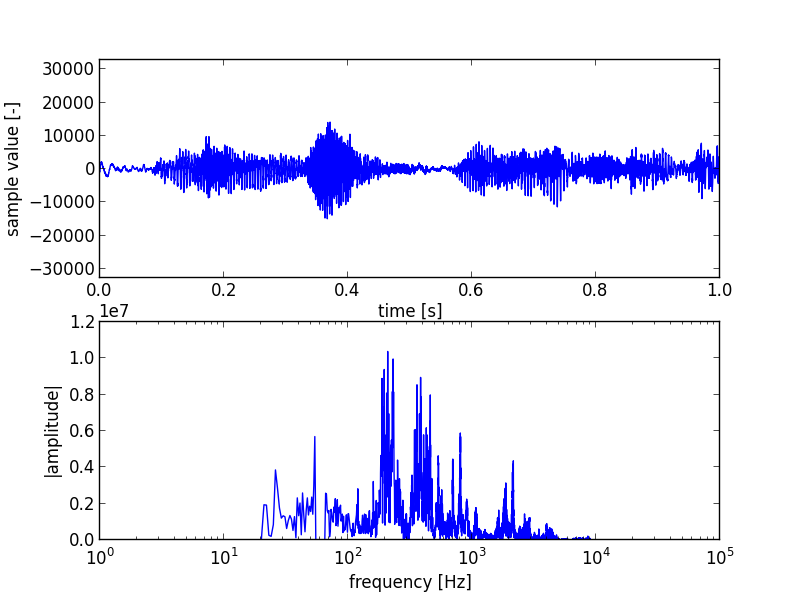
\includegraphics[width=1\textwidth]{fourier}
\caption{Fourier transform applied over a sound}
\label{fig:fourier}
\end{figure}


The \emph{Nyquist–Shannon} sampling theorem states that a signal can be exactly reconstructed from its samples if the sampling frequency is greater than twice the highest frequency component in the signal. In practice, the sampling frequency is often significantly higher than twice the Nyquist frequency\cite{note5}. In this case, where the target range is about 20-26 khz, a sampling  rate of 48000 samples/second is almost at the limit, meaning that some higher frequencies might be omitted and loss of accuracy, so a higher sampling rate was chosen: 96000 samples/second.


\section{Just a little bit of anatomy}
A basic measure of hearing is afforded by an audiogram (fig \ref{fig:human_hearing}), a graph of the absolute threshold of hearing (minimum discernible sound level) at various frequencies throughout an organism's nominal hearing range. The commonly stated range of human hearing is 20 Hz to 20 kHz.Under ideal laboratory conditions, humans can hear sound as low as 12 Hz and as high as 28 kHz, though the threshold increases sharply at 15 kHz in adults. Humans are most sensitive to (i.e. able to discern at lowest intensity) frequencies between 2,000 and 5,000 Hz. Individual hearing range varies according to the general condition of a human's ears and nervous system. The range shrinks during life, usually beginning at around age of eight with the upper frequency limit being reduced. Women typically experience a lesser degree of hearing loss than men, with a later onset. Men have approximately 5 to 10 dB greater loss in the upper frequencies by age 40\cite{note6}.
This practical application of this work will focus on the range of 15-24 kHz with variable  sound amplitude as a program doesn't need a very high signal amplitude to recognize it. Preferably the lower end of the encoding range should be as high as possible to exclude the possibility of certain humans hearing the noise added, but due to hardware limitations this threshold shouldn't pass 24-25 kHz (to be further discussed in this paper).

As the range of human hearing is variable from one person to another, there exists the possiblity of some persons hearing certain anomalies at the lower end of the frequency specter used in this method, but the application features a mechanism to prevent such detections by raisign the overall height of the frequencies used.

\begin{figure}[h]
\centering
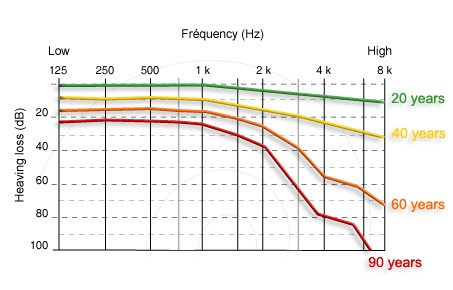
\includegraphics[width=1\textwidth]{human_hearing}
\caption{Human hearing audiograms based on age\cite{note7} MUST CHANGE BAD!!}
\label{fig:human_hearing}
\end{figure}

\chapter{The application}
For proving the concept of hiding information using high frequency signals, an python application was implemented
\section{Chosen method}
\section{Environment}
\subsection{File encoding formats}
\subsubsection{WAV format}
\subsection{Python programming language}
\subsection{Matlab and matplotlib integrtion in python}
\subsection{Numpy}
\subsection{Tkinter UI development in Python}


\section{Limitations}
\subsection{Hardware limitations}
\subsection{Software limitations}

\section{Further improvements}

\chapter{Comparison with existent methods}

\section{Other techniques}
The number of other methods used for hiding messages has seen a continous increase over the years. We will present only some of the most frequent used in audio frequency, but this list is far from being exhaustive. Each of this methods comes with its advantages or disadvantages which will be discussed later.
\subsection{Structural methods}
\subsection{LSB \emph{(least significant byte}) method}
\subsection{Phase coding}
\section{Advantages/disadvantages}



\begin{thebibliography}{6}
\bibitem{note1}
Katzenbeisser, S., Petitcolas, F.A.P.: Information Hiding: Techniques for steganography 
and digital watermarking. Artech House, Boston (1999) 
\bibitem{note2}
Mahendra Kumar Pandey, Girish Parmar, and Sanjay Patsariya:An Effective Way to Hide the Secret Audio File Using 
High Frequency Manipulation (2011)
\bibitem{note3}
Ahmed Hussain Ali,Mohd Rosmadi Mokhtar and LoayEdwar George: A Review on Audio Steganography Techniques (2015)
\bibitem{note4}
Pahati, OJ (2001-11-29). "Confounding Carnivore: How to Protect Your Online Privacy". AlterNet. Archived from the original on 2007-07-16. Retrieved 2008-09-02.
\bibitem{note5}
Candes, E. J., Wakin, M. B. (2008). An Introduction To Compressive Sampling. IEEE Signal Processing Magazine, 25(2), 21-30. doi:10.1109/MSP.2007.914731
\bibitem{note6}
Marler, Peter (2004). Nature's Music: The Science of Birdsong. Academic Press Inc. p. 207. ISBN 978-0124730700
\bibitem{note7}
Stéphan Blatrix, www.neuroreille.com, 1999
\end{thebibliography}


\end{document}